\begin{enumerate}[label=\thechapter.\arabic*,ref=\thechapter.\theenumi]

\item Consider a unity-gain negative feedback system consisting of the plant $G\brak{s}$  and a proportional-integral controller. Let the proportional gain and integral
gain be 3 and 1, respectively. For a unit step reference input, the final values of the
controller output and the plant output, respectively, are
\begin{align}
    G\brak{s} = \frac{1}{\brak{s-1}} \notag
\end{align}\hfill (GATE EE 2023)\\
\solution 
%% Run LaTeX on this file several times to get Table of Contents,
%% cross-references, and citations.

\documentclass[11pt]{book}
\usepackage{gvv-book}
\usepackage{gvv}
%\usepackage{Wiley-AuthoringTemplate}
\usepackage[sectionbib,authoryear]{natbib}% for name-date citation comment the below line
%\usepackage[sectionbib,numbers]{natbib}% for numbered citation comment the above line

%%********************************************************************%%
%%       How many levels of section head would you like numbered?     %%
%% 0= no section numbers, 1= section, 2= subsection, 3= subsubsection %%
\setcounter{secnumdepth}{3}
%%********************************************************************%%
%%**********************************************************************%%
%%     How many levels of section head would you like to appear in the  %%
%%				Table of Contents?			%%
%% 0= chapter, 1= section, 2= subsection, 3= subsubsection titles.	%%
\setcounter{tocdepth}{2}
%%**********************************************************************%%

%\includeonly{ch01}
\makeindex

\begin{document}

\frontmatter
%%%%%%%%%%%%%%%%%%%%%%%%%%%%%%%%%%%%%%%%%%%%%%%%%%%%%%%%%%%%%%%%
%% Title Pages
%% Wiley will provide title and copyright page, but you can make
%% your own titlepages if you'd like anyway
%% Setting up title pages, type in the appropriate names here:

\booktitle{Signal Processing }

\subtitle{Through GATE}

\AuAff{G. V. V. Sharma}


%% \\ will start a new line.
%% You may add \affil{} for affiliation, ie,
%\authors{Robert M. Groves\\
%\affil{Universitat de les Illes Balears}
%Floyd J. Fowler, Jr.\\
%\affil{University of New Mexico}
%}

%% Print Half Title and Title Page:
%\halftitlepage
\titlepage

%%%%%%%%%%%%%%%%%%%%%%%%%%%%%%%%%%%%%%%%%%%%%%%%%%%%%%%%%%%%%%%%
%% Copyright Page

\begin{copyrightpage}{2024}
%Title, etc
\end{copyrightpage}

% Note, you must use \ to start indented lines, ie,
% 
% \begin{copyrightpage}{2004}
% Survey Methodology / Robert M. Groves . . . [et al.].
% \       p. cm.---(Wiley series in survey methodology)
% \    ``Wiley-Interscience."
% \    Includes bibliographical references and index.
% \    ISBN 0-471-48348-6 (pbk.)
% \    1. Surveys---Methodology.  2. Social 
% \  sciences---Research---Statistical methods.  I. Groves, Robert M.  II. %
% Series.\\

% HA31.2.S873 2004
% 001.4'33---dc22                                             2004044064
% \end{copyrightpage}

%%%%%%%%%%%%%%%%%%%%%%%%%%%%%%%%%%%%%%%%%%%%%%%%%%%%%%%%%%%%%%%%
%% Only Dedication (optional) 

%\dedication{To my parents}

\tableofcontents

%\listoffigures %optional
%\listoftables  %optional

%% or Contributor Page for edited books
%% before \tableofcontents

%%%%%%%%%%%%%%%%%%%%%%%%%%%%%%%%%%%%%%%%%%%%%%%%%%%%%%%%%%%%%%%%
%  Contributors Page for Edited Book
%%%%%%%%%%%%%%%%%%%%%%%%%%%%%%%%%%%%%%%%%%%%%%%%%%%%%%%%%%%%%%%%

% If your book has chapters written by different authors,
% you'll need a Contributors page.

% Use \begin{contributors}...\end{contributors} and
% then enter each author with the \name{} command, followed
% by the affiliation information.

% \begin{contributors}
% \name{Masayki Abe,} Fujitsu Laboratories Ltd., Fujitsu Limited, Atsugi, Japan
%
% \name{L. A. Akers,} Center for Solid State Electronics Research, Arizona State University, Tempe, Arizona
%
% \name{G. H. Bernstein,} Department of Electrical and Computer Engineering, University of Notre Dame, Notre Dame, South Bend, Indiana; formerly of
% Center for Solid State Electronics Research, Arizona
% State University, Tempe, Arizona 
% \end{contributors}

%%%%%%%%%%%%%%%%%%%%%%%%%%%%%%%%%%%%%%%%%%%%%%%%%%%%%%%%%%%%%%%%
% Optional Foreword:

%\begin{foreword}
%\lipsum[1-2]
%\end{foreword}

%%%%%%%%%%%%%%%%%%%%%%%%%%%%%%%%%%%%%%%%%%%%%%%%%%%%%%%%%%%%%%%%
% Optional Preface:

%\begin{preface}
%\lipsum[1-1]
%\prefaceauthor{}
%\where{place\\
% date}
%\end{preface}

% ie,
% \begin{preface}
% This is an example preface.
% \prefaceauthor{R. K. Watts}
% \where{Durham, North Carolina\\
% September, 2004}

%%%%%%%%%%%%%%%%%%%%%%%%%%%%%%%%%%%%%%%%%%%%%%%%%%%%%%%%%%%%%%%%
% Optional Acknowledgments:

%\acknowledgments
%\lipsum[1-2]
%\authorinitials{I. R. S.}  

%%%%%%%%%%%%%%%%%%%%%%%%%%%%%%%%
%% Glossary Type of Environment:

% \begin{glossary}
% \term{<term>}{<description>}
% \end{glossary}

%%%%%%%%%%%%%%%%%%%%%%%%%%%%%%%%
%\begin{acronyms}
%\acro{ASTA}{Arrivals See Time Averages}
%\acro{BHCA}{Busy Hour Call Attempts}
%\acro{BR}{Bandwidth Reservation}
%\acro{b.u.}{bandwidth unit(s)}
%\acro{CAC}{Call / Connection Admission Control}
%\acro{CBP}{Call Blocking Probability(-ies)}
%\acro{CCS}{Centum Call Seconds}
%\acro{CDTM}{Connection Dependent Threshold Model}
%\acro{CS}{Complete Sharing}
%\acro{DiffServ}{Differentiated Services}
%\acro{EMLM}{Erlang Multirate Loss Model}
%\acro{erl}{The Erlang unit of traffic-load}
%\acro{FIFO}{First in - First out}
%\acro{GB}{Global balance}
%\acro{GoS}{Grade of Service}
%\acro{ICT}{Information and Communication Technology}
%\acro{IntServ}{Integrated Services}
%\acro{IP}{Internet Protocol}
%\acro{ITU-T}{International Telecommunication Unit -- Standardization sector}
%\acro{LB}{Local balance}
%\acro{LHS}{Left hand side}
%\acro{LIFO}{Last in - First out}
%\acro{MMPP}{Markov Modulated Poisson Process}
%\acro{MPLS}{Multiple Protocol Labeling Switching}
%\acro{MRM}{Multi-Retry Model}
%\acro{MTM}{Multi-Threshold Model}
%\acro{PASTA}{Poisson Arrivals See Time Averages}
%\acro{PDF}{Probability Distribution Function}
%\acro{pdf}{probability density function}
%\acro{PFS}{Product Form Solution}
%\acro{QoS}{Quality of Service}
%\acro{r.v.}{random variable(s)}
%\acro{RED}{random early detection}
%\acro{RHS}{Right hand side}
%\acro{RLA}{Reduced Load Approximation}
%\acro{SIRO}{service in random order}
%\acro{SRM}{Single-Retry Model}
%\acro{STM}{Single-Threshold Model}
%\acro{TCP}{Transport Control Protocol}
%\acro{TH}{Threshold(s)}
%\acro{UDP}{User Datagram Protocol}
%\end{acronyms}

\setcounter{page}{1}

\begin{introduction}
This book provides solutions to signal processing problems in GATE.

\end{introduction}

\mainmatter

\chapter{Harmonics}
\begin{enumerate}[label=\thechapter.\arabic*,ref=\thechapter.\theenumi]



\end{enumerate}

\chapter{Filters}
\begin{enumerate}[label=\thechapter.\arabic*,ref=\thechapter.\theenumi]
\item
For the circuit given below, choose the angular frequency $ \omega_0$ at which voltage across capacitor has maximum amplitude?
\begin{figure}[h!]
    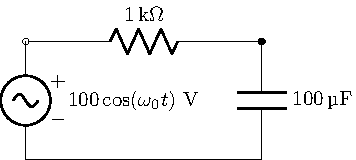
\includegraphics[width = 0.5\columnwidth]{2023/BM/16/figs/c_fig1.pdf}
    \caption{circuit }
    \centering
    \label{fig: bm_16_fig_1}
\end{figure}
\begin{enumerate}
    \item[(A)] 1000
    \item[(B)] 100
    \item[(C)] 1
    \item[(D)] 0   
\end{enumerate}
\hfill(GATE BM 2023 Question 16)\\

\solution
\iffalse
\let\negmedspace\undefined
\let\negthickspace\undefined
\documentclass[journal,12pt,twocolumn]{IEEEtran}
\usepackage{cite}
\usepackage{amsmath,amssymb,amsfonts,amsthm}
\usepackage{algorithmic}
\usepackage{graphicx}
\usepackage{textcomp}
\usepackage{xcolor}
\usepackage{txfonts}
\usepackage{listings}
\usepackage{enumitem}
\usepackage{mathtools}
\usepackage{gensymb}
\usepackage{comment}
\usepackage[breaklinks=true]{hyperref}
\usepackage{tkz-euclide}
\usepackage{listings}
\usepackage{gvv}
\def\inputGnumericTable{}
\usepackage[latin1]{inputenc}
\usepackage{color}
\usepackage{array}
\usepackage{longtable}
\usepackage{calc}
\usepackage{multirow}
\usepackage{hhline}
\usepackage{ifthen}
\usepackage{lscape}

\newtheorem{theorem}{Theorem}[section]
\newtheorem{problem}{Problem}
\newtheorem{proposition}{Proposition}[section]
\newtheorem{lemma}{Lemma}[section]
\newtheorem{corollary}[theorem]{Corollary}
\newtheorem{example}{Example}[section]
\newtheorem{definition}[problem]{Definition}
\newcommand{\BEQA}{\begin{eqnarray}}
\newcommand{\EEQA}{\end{eqnarray}}
\newcommand{\define}{\stackrel{\triangle}{=}}
\theoremstyle{remark}
\newtheorem{rem}{Remark}
\begin{document}

\bibliographystyle{IEEEtran}
\vspace{3cm}

\title{GATE -BM 16}
\author{EE23BTECH11057 - Shakunaveti Sai Sri Ram Varun$^{}$% &lt;-this % stops a space
}
\maketitle
\newpage
\bigskip
\vspace{2cm}
\textbf{Question: }
For the circuit given below, choose the angular frequency $ \omega_0$ at which voltage across capacitor has maximum amplitude?
\begin{figure}[h!]
    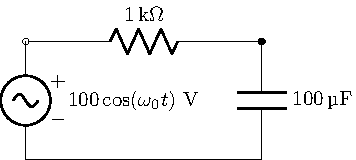
\includegraphics[width = \columnwidth]{2023/BM/16/figs/c_fig1.pdf}
    \caption{circuit }
    \centering
    \label{fig: bm_16_fig_1}
\end{figure}\\
\begin{enumerate}
    \item[(A)] 1000\\
    \item[(B)] 100\\
    \item[(C)] 1\\
    \item[(D)] 0   
\end{enumerate}
\hfill(GATE BM 2023 question 16)\\
\textbf{Solution}:\\
\fi
\begin{table}[h!] 
\centering
\input{2023/BM/16/tables/table1}
\caption{input values}
\label{tab: table-bm16}
\end{table}

\begin{align}
V_c\brak{s}&= \frac{V_1\brak{s}\frac{1}{sC}}{R+\frac{1}{sC}}\\
\implies H\brak{s} &= \frac{1}{1+ sRC}\\
\implies H\brak{j\omega} &= \frac{1}{1+j\omega RC}\\
|H\brak{j\omega}| &= \frac{1}{\sqrt{1+\brak{\omega RC}^2}}
\end{align}
\begin{figure}[h!]
    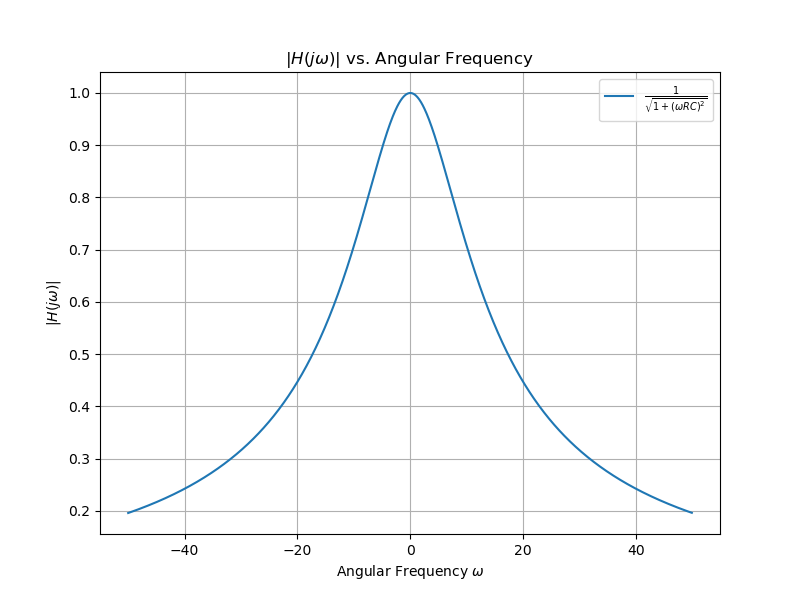
\includegraphics[width = \columnwidth]{2023/BM/16/figs/Figure_1.png}
    \caption{$ |H\brak{j\omega}|$ }
    \centering
    \label{fig: bm_16_fig_2}
\end{figure}


\begin{figure}[h!]
    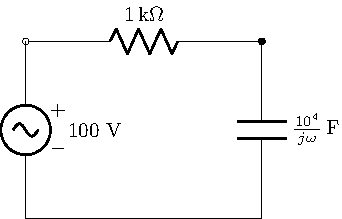
\includegraphics[width = \columnwidth]{2023/BM/16/figs/c_fig2.pdf}
    \caption{circuit in $ \omega$-domain }
    \centering
    \label{fig: bm_16_fig_3}
\end{figure}

\begin{align}
v_c\brak{t}&= \frac{100}{\sqrt{1+\brak{\omega_o RC}^2}}\brak{\cos{\omega_o t + \arctan\brak{\frac{1}{\omega_o RC}}}}
\end{align}
Maximum amplitude of $ v_c\brak{t}$ occurs at $ \omega_o=0$
\begin{align}
\therefore \omega_o =0
\end{align}
$ \therefore$ maximum value of $ v_c\brak{t}$ at steady state is $ 100$ Volts.

\newpage
\item
In the following circuit, the switch S is open for $t < 0$ and closed for $t \ge 0$.
What is the steady state voltage (in Volts) across the capacitor when the switch is closed?
\begin{figure}[h!]
    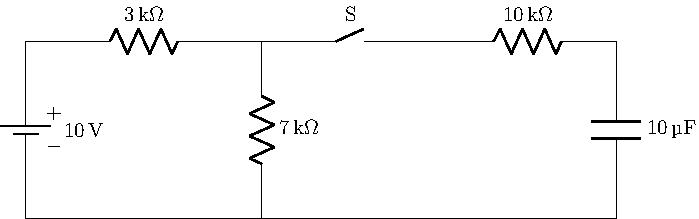
\includegraphics[width = 0.7\columnwidth]{2023/BM/30/figs/c_fig1.pdf}
    \caption{circuit }
    \centering
    \label{fig:bm_30_fig_1}
\end{figure}
\hfill(GATE BM 2023 Question 30)\\
\item 
A finite impulse response (FIR) filter has only two non-zero samples in its impulse response $h[n]$, namely $h[0] = h[1] = 1$. The Discrete Time Fourier Transform (DTFT) of $h[n]$ equals $H(e^{j\omega})$, as a function of the normalized angular frequency $\omega$. For the range $\abs{\omega} \leq \pi$, $\abs{H(e^{j\omega})}$ is equal to
\begin{enumerate}
	\item[(A)] $2\abs{\cos(\omega)}$
	\item[(B)] $2\abs{\sin(\omega)}$
	\item[(C)] $2\abs{\cos(\frac{\omega}{2})}$
	\item[(D)] $2\abs{\sin(\frac{\omega}{2})}$
\end{enumerate}
\hfill(GATE BM 2023 Question 17) \\
\item
For the circuit shown,if $i=\sin 1000t$, the instantaneous value of the Thevenin's voltage(in volts) across the terminals a anb b at time t=5ms is\\[2pt]

\begin{circuitikz}[american voltages,american currents]
    % Draw the circuit components
    \draw (0,0) -- (2,0);
    \draw (2,2) to [resistor,l=$10\Omega$] (2,4);
    \draw (2,4) -- (0,4);
    \draw (2,0) to [capacitor,l=$-j10\Omega$,-,i_=$i_x$] (2,2);
    \draw (2,0) -- (5,0);
    \draw (5,0) to[inductor,l=$j10\Omega$] (5,2);
    \draw (5,2) to [resistor,l=$10\Omega$] (5,4);
  \draw (5,4) to [cV,l^=$4i_x$,invert] (2,4);
  \draw (5,4) -- (6,4);
  \draw (6,4) to[I,l=$\sin 1000t$,invert] (6,0);
  \draw (6,0) -- (5,0);
   \node[circle,fill=black,inner sep=1.5pt,label=above:a] at (0,0) {};
    \node[circle,fill=black,inner sep=1.5pt,label=above:b] at (0,4) {};
    \end{circuitikz}
    \hfill(GATE EE 2023 Question 51) \\
    \pagebreak

    \item In the circuit shown ,$\omega=100\pi\text{rads/s}$, R1=R2=$2.2\Omega$ and L=$7\text{mH}$. the capacitance $\text{C}$ for which $Y_{in}$ is purely real is  $\text{mF}$ \\
	\begin{center}
	\begin{circuitikz} \centering \draw 
		(0,4) to[sinusoidal voltage source, l=$V_{0}$cos($\omega$t)] (0,0)
		(0,4) to[short] (4,4)
		(4,4) to[resistor, l=$R_1$ ] (4,2)
		(4,2) to[inductor, l= $\text{L} $] (4,0) to[short ] (0,0)
		(8,4)  to[short] (4,4)
		(8,4) to[resistor, l= $R_2$] (8,2) to[capacitor,l=$\text{C}$] (8,0) to (4,0);
	\end{circuitikz}
	\end{center}
\hfill(GATE IN 2023 Q46)\\
\solution

\pagebreak
\item An input voltage in the form of a square wave of frequency $1\, kHz$ is given to a circuit, which results in the output shown schematically below. Which one of the following options is the CORRECT representation of the circuit? \hfill(GATE PH 2023 Q37)
\begin{figure}[!h]
    \centering
    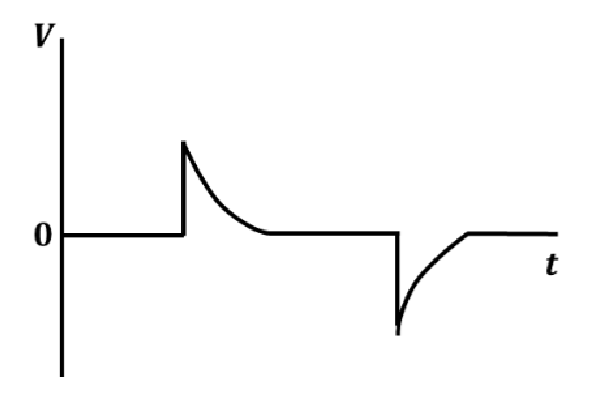
\includegraphics[width = 0.6\columnwidth]{2023/PH/37/figs/question.png}
    \caption{}
\end{figure}

\begin{enumerate}[label = (\alph*)]
    \item 
    \begin{figure}[!h]
        \centering
	    \resizebox{0.2\textwidth}{!}{\begin{circuitikz}
    \draw(0, 0) to[short,*-*] ++ (4,0);
\draw (0,2) to[C,l=$0.1\mu F$, *-*] ++ (3,0) coordinate(a);
\draw (a) to[short,-*] ++ (1,0);
\draw (a) to[R, l_=$0.5k\Omega$,*-] ++(0,-2);

% Voltage labels
\draw (0,2) to[open,l_=V$_{in}$] ++(0,-2);
\draw (4,2) to[open,l=V$_{out}$] ++(0,-2);
\end{circuitikz}

}
	\label{optA_gate.ph.23.37}
    \end{figure}

    \item 
    \begin{figure}[!h]
        \centering
        \resizebox{0.2\textwidth}{!}{\begin{circuitikz}
    \draw(0, 0) to[short,*-*] ++ (4,0);
\draw (0,2) to[C,l=$1\mu F$, *-*] ++ (3,0) coordinate(a);
\draw (a) to[short,-*] ++ (1,0);
\draw (a) to[R, l_=$5k\Omega$,*-] ++(0,-2);

% Voltage labels
\draw (0,2) to[open,l_=V$_{in}$] ++(0,-2);
\draw (4,2) to[open,l=V$_{out}$] ++(0,-2);
\end{circuitikz}

}
        \label{optB_gate.ph.23.37}
    \end{figure}

    \item 
    \begin{figure}[!h]
        \centering
        \resizebox{0.2\textwidth}{!}{\begin{circuitikz}
    \draw(0, 0) to[short,*-*] ++ (4,0);
\draw (0,2) to[R, l = $0.5k\Omega$, *-] ++ (3,0) coordinate(a);
\draw (a) to[short,-*] ++ (1,0);
\draw (a) to[C,l_=$0.1\mu F$,*-*] ++(0,-2);

% Voltage labels
\draw (0,2) to[open,l_=V$_{in}$] ++(0,-2);
\draw (4,2) to[open,l=V$_{out}$] ++(0,-2);
\end{circuitikz}

}
        \label{optC_gate.ph.23.37}
    \end{figure}

    \item 
    \begin{figure}[!h]
        \centering
        \resizebox{0.2\textwidth}{!}{\begin{circuitikz}
    \draw(0, 0) to[short,*-*] ++ (4,0);
\draw (0,2) to[R, l = $5k\Omega$, *-] ++ (3,0) coordinate(a);
\draw (a) to[short,-*] ++ (1,0);
\draw (a) to[C,l_=$1\mu F$,*-*] ++(0,-2);

% Voltage labels
\draw (0,2) to[open,l_=V$_{in}$] ++(0,-2);
\draw (4,2) to[open,l=V$_{out}$] ++(0,-2);
\end{circuitikz}

}
        \label{optD_gate.ph.23.37}
    \end{figure}
\end{enumerate} \hfill(GATE 2023 PH 37)
\solution

\pagebreak
\pagebreak

\item In the circuit shown below, switch S was closed for long time. If the switch is opened at $t=0$, the  maximum magnitude of the voltage $V_R$ , in volts is (rounded off to the nearest integer)\hfill{(GATE 2023 EC 35)}\\
\begin{figure}[h!]
    \centering
    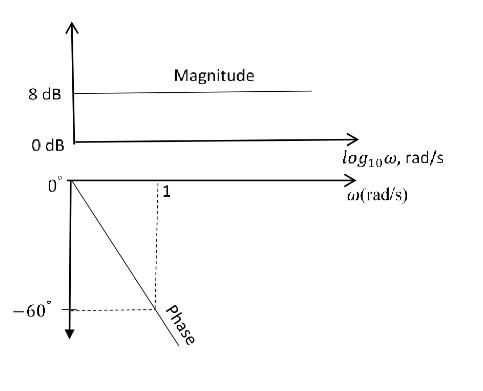
\includegraphics[width=1\linewidth]{2023/EC/35/figs/gate.png}
    \caption{ }
\end{figure}
\solution
\pagebreak
\item A signal $x\brak{t}=2\cos{(180\pi t)}\cos{(60\pi t)}$ is sampled at 200 Hz and then passed through an ideal low pass filter having cut-off frequency of 100 Hz.\\
The maximum Frequency present in the filtered  signal in Hz is \rule{1cm}{0.5mm} (Round off to the nearest integer.) \hfill (GATE 2023 EE)
\solution
\pagebreak

\item The op amps in the circuit are ideal. The input signals are $V_{S1} = 3 + 0.10 \sin(300t), \text{V}$ and $V_{S2} = -2 + 0.11 \sin(300t)\, \text{V}$. The average value of the voltage $V_0$ is \underline{\hspace{1cm}} volts (rounded off to two decimal places).

\begin{figure}[ht]
\centering
\resizebox{0.55\columnwidth}{!}{\begin{circuitikz}

% Lines
\draw (-2.5,2.5) -- (0.5,2.5);
\draw (0.5,3) -- (0.5,1);
\draw (0.5,1.5) -- (0,1.5);
\draw (0,1.5) -- (0,0);
\draw (-2.5,-4) -- (0.5,-4);
\draw (0.5,-4.5) -- (0.5,-2.5);
\draw (0.5,-3) -- (0,-3);
\draw (0,-3) -- (0,-1.5);
\draw (0.5,3) -- (2,2);
\draw (0.5,1) -- (2,2);
\draw (2,2) -- (3.5,2);
\draw (3.5,2) -- (5.5,2);
\draw (3.5,2) -- (3.5,1.5);
\draw (0.5,-2.5) -- (2,-3.5);
\draw (0.5,-4.5) -- (2,-3.5);
\draw (2,-3.5) -- (3.5,-3.5);
\draw (3.5,-3.5) -- (3.5,-3);
\draw (3.5,-3.5) -- (5.5,-3.5);
\draw (5.5,-3.5) -- (5.5,-2.25);
\draw (5.5,2) -- (5.5,0.75);
\draw (5.5,-0.75) -- (6.5,-0.75);
\draw (0,0) -- (3.5,0);
\draw (0,-1.5) -- (3.5,-1.5);
\draw (6.5,-1.5) -- (6.5,-2.5);
\draw (6.25,-2.5) -- (6.75,-2.5);
\draw (6.3,-2.55) -- (6.7,-2.55);


% Resistors
\draw (3.5,1.5) to [resistor] (3.5,0);
\draw (3.5,0) to [resistor] (3.5,-1.5);
\draw (3.5,-1.5) to [resistor] (3.5,-3);
\draw (5.5,0.75) to [resistor] (5.5,-0.75);
\draw (5.5,-0.75) to [resistor] (5.5,-2.25);

% Labels
\node at (-3,2.5) {$V_{S1}$};
\node at (-3,-4) {$V_{S2}$};
\node at (0.75,2.5) {+};
\node at (0.75,1.5) {-};
\node at (0.75,-3) {-};
\node at (0.75,-4) {+};
\node at (7,-0.75) {$V_o$};
\node at (4.25,0.75) {R};
\node at (4.25,-0.75) {R};
\node at (4.25,-2.25) {R};
\node at (6.25,0) {R};
\node at (6.25,-1.5) {R};
\node at (6.75,-0.8) {+};
\node at (6.75,-1.5) {-};

% Dot 
\filldraw (6.5,-0.75) circle [radius=0.05];
\fill (6.5,-1.5) circle [radius=0.05]; 

\end{circuitikz}

}
\end{figure}
\end{figure}
\hfill{(GATE IN 2023)}\\
\solution
\pagebreak
\end{enumerate}

\chapter{ Z-transform}
\chapter{Systems}

\begin{enumerate}[label=\thechapter.\arabic*,ref=\thechapter.\theenumi]

\item Consider a unity-gain negative feedback system consisting of the plant $G\brak{s}$  and a proportional-integral controller. Let the proportional gain and integral
gain be 3 and 1, respectively. For a unit step reference input, the final values of the
controller output and the plant output, respectively, are
\begin{align}
    G\brak{s} = \frac{1}{\brak{s-1}} \notag
\end{align}\hfill (GATE EE 2023)\\
\solution 
%% Run LaTeX on this file several times to get Table of Contents,
%% cross-references, and citations.

\documentclass[11pt]{book}
\usepackage{gvv-book}
\usepackage{gvv}
%\usepackage{Wiley-AuthoringTemplate}
\usepackage[sectionbib,authoryear]{natbib}% for name-date citation comment the below line
%\usepackage[sectionbib,numbers]{natbib}% for numbered citation comment the above line

%%********************************************************************%%
%%       How many levels of section head would you like numbered?     %%
%% 0= no section numbers, 1= section, 2= subsection, 3= subsubsection %%
\setcounter{secnumdepth}{3}
%%********************************************************************%%
%%**********************************************************************%%
%%     How many levels of section head would you like to appear in the  %%
%%				Table of Contents?			%%
%% 0= chapter, 1= section, 2= subsection, 3= subsubsection titles.	%%
\setcounter{tocdepth}{2}
%%**********************************************************************%%

%\includeonly{ch01}
\makeindex

\begin{document}

\frontmatter
%%%%%%%%%%%%%%%%%%%%%%%%%%%%%%%%%%%%%%%%%%%%%%%%%%%%%%%%%%%%%%%%
%% Title Pages
%% Wiley will provide title and copyright page, but you can make
%% your own titlepages if you'd like anyway
%% Setting up title pages, type in the appropriate names here:

\booktitle{Signal Processing }

\subtitle{Through GATE}

\AuAff{G. V. V. Sharma}


%% \\ will start a new line.
%% You may add \affil{} for affiliation, ie,
%\authors{Robert M. Groves\\
%\affil{Universitat de les Illes Balears}
%Floyd J. Fowler, Jr.\\
%\affil{University of New Mexico}
%}

%% Print Half Title and Title Page:
%\halftitlepage
\titlepage

%%%%%%%%%%%%%%%%%%%%%%%%%%%%%%%%%%%%%%%%%%%%%%%%%%%%%%%%%%%%%%%%
%% Copyright Page

\begin{copyrightpage}{2024}
%Title, etc
\end{copyrightpage}

% Note, you must use \ to start indented lines, ie,
% 
% \begin{copyrightpage}{2004}
% Survey Methodology / Robert M. Groves . . . [et al.].
% \       p. cm.---(Wiley series in survey methodology)
% \    ``Wiley-Interscience."
% \    Includes bibliographical references and index.
% \    ISBN 0-471-48348-6 (pbk.)
% \    1. Surveys---Methodology.  2. Social 
% \  sciences---Research---Statistical methods.  I. Groves, Robert M.  II. %
% Series.\\

% HA31.2.S873 2004
% 001.4'33---dc22                                             2004044064
% \end{copyrightpage}

%%%%%%%%%%%%%%%%%%%%%%%%%%%%%%%%%%%%%%%%%%%%%%%%%%%%%%%%%%%%%%%%
%% Only Dedication (optional) 

%\dedication{To my parents}

\tableofcontents

%\listoffigures %optional
%\listoftables  %optional

%% or Contributor Page for edited books
%% before \tableofcontents

%%%%%%%%%%%%%%%%%%%%%%%%%%%%%%%%%%%%%%%%%%%%%%%%%%%%%%%%%%%%%%%%
%  Contributors Page for Edited Book
%%%%%%%%%%%%%%%%%%%%%%%%%%%%%%%%%%%%%%%%%%%%%%%%%%%%%%%%%%%%%%%%

% If your book has chapters written by different authors,
% you'll need a Contributors page.

% Use \begin{contributors}...\end{contributors} and
% then enter each author with the \name{} command, followed
% by the affiliation information.

% \begin{contributors}
% \name{Masayki Abe,} Fujitsu Laboratories Ltd., Fujitsu Limited, Atsugi, Japan
%
% \name{L. A. Akers,} Center for Solid State Electronics Research, Arizona State University, Tempe, Arizona
%
% \name{G. H. Bernstein,} Department of Electrical and Computer Engineering, University of Notre Dame, Notre Dame, South Bend, Indiana; formerly of
% Center for Solid State Electronics Research, Arizona
% State University, Tempe, Arizona 
% \end{contributors}

%%%%%%%%%%%%%%%%%%%%%%%%%%%%%%%%%%%%%%%%%%%%%%%%%%%%%%%%%%%%%%%%
% Optional Foreword:

%\begin{foreword}
%\lipsum[1-2]
%\end{foreword}

%%%%%%%%%%%%%%%%%%%%%%%%%%%%%%%%%%%%%%%%%%%%%%%%%%%%%%%%%%%%%%%%
% Optional Preface:

%\begin{preface}
%\lipsum[1-1]
%\prefaceauthor{}
%\where{place\\
% date}
%\end{preface}

% ie,
% \begin{preface}
% This is an example preface.
% \prefaceauthor{R. K. Watts}
% \where{Durham, North Carolina\\
% September, 2004}

%%%%%%%%%%%%%%%%%%%%%%%%%%%%%%%%%%%%%%%%%%%%%%%%%%%%%%%%%%%%%%%%
% Optional Acknowledgments:

%\acknowledgments
%\lipsum[1-2]
%\authorinitials{I. R. S.}  

%%%%%%%%%%%%%%%%%%%%%%%%%%%%%%%%
%% Glossary Type of Environment:

% \begin{glossary}
% \term{<term>}{<description>}
% \end{glossary}

%%%%%%%%%%%%%%%%%%%%%%%%%%%%%%%%
%\begin{acronyms}
%\acro{ASTA}{Arrivals See Time Averages}
%\acro{BHCA}{Busy Hour Call Attempts}
%\acro{BR}{Bandwidth Reservation}
%\acro{b.u.}{bandwidth unit(s)}
%\acro{CAC}{Call / Connection Admission Control}
%\acro{CBP}{Call Blocking Probability(-ies)}
%\acro{CCS}{Centum Call Seconds}
%\acro{CDTM}{Connection Dependent Threshold Model}
%\acro{CS}{Complete Sharing}
%\acro{DiffServ}{Differentiated Services}
%\acro{EMLM}{Erlang Multirate Loss Model}
%\acro{erl}{The Erlang unit of traffic-load}
%\acro{FIFO}{First in - First out}
%\acro{GB}{Global balance}
%\acro{GoS}{Grade of Service}
%\acro{ICT}{Information and Communication Technology}
%\acro{IntServ}{Integrated Services}
%\acro{IP}{Internet Protocol}
%\acro{ITU-T}{International Telecommunication Unit -- Standardization sector}
%\acro{LB}{Local balance}
%\acro{LHS}{Left hand side}
%\acro{LIFO}{Last in - First out}
%\acro{MMPP}{Markov Modulated Poisson Process}
%\acro{MPLS}{Multiple Protocol Labeling Switching}
%\acro{MRM}{Multi-Retry Model}
%\acro{MTM}{Multi-Threshold Model}
%\acro{PASTA}{Poisson Arrivals See Time Averages}
%\acro{PDF}{Probability Distribution Function}
%\acro{pdf}{probability density function}
%\acro{PFS}{Product Form Solution}
%\acro{QoS}{Quality of Service}
%\acro{r.v.}{random variable(s)}
%\acro{RED}{random early detection}
%\acro{RHS}{Right hand side}
%\acro{RLA}{Reduced Load Approximation}
%\acro{SIRO}{service in random order}
%\acro{SRM}{Single-Retry Model}
%\acro{STM}{Single-Threshold Model}
%\acro{TCP}{Transport Control Protocol}
%\acro{TH}{Threshold(s)}
%\acro{UDP}{User Datagram Protocol}
%\end{acronyms}

\setcounter{page}{1}

\begin{introduction}
This book provides solutions to signal processing problems in GATE.

\end{introduction}

\mainmatter

\chapter{Harmonics}
\input{2023/harmonics.tex}
\chapter{Filters}
\input{2023/filters.tex}
\chapter{ Z-transform}
\chapter{Systems}
\input{2023/systems.tex}
\chapter{Sequences}
\input{2023/sequences.tex}
\chapter{Sampling}
\input{2023/sampling.tex}
\chapter{Contour Integration}
\input{2023/contour.tex}
\chapter{Laplace Transform}
 \input{2023/laplace.tex}
\chapter{Fourier transform}
 \input{2023/fourier.tex}
\backmatter
\appendix
\iffalse
\chapter{ Convolution}
\chapter{ Z-transform}
\fi
\latexprintindex

\end{document}

 

\newpage

\item Level \brak{h} in a steam boiler is controlled by manipulating the flow rate \brak{F} of the break-up(fresh) water using a proportional \brak{P} controller. The transfer function between the output and the manipulated input is   \\
$$ \frac{h\brak{s}}{F\brak{s}}=\frac{0.25\brak{1-s}}{s\brak{2s+1}} $$   \\
The measurement and the valve transfer functions are both equal to 1. A process engineer wants to tune the controller so that the closed loop response gives the decaying oscillations under the servo mode. Which one of the following is the CORRECT value of the controller gain to be used by the engineer? \\
\begin{enumerate}[label=(\alph*)]
    \item $0.25$
    \item $2$
    \item $4$
    \item $6$
\end{enumerate} \hfill{GATE CH 2023} \\

\solution
\newpage
\item \input{2023/ME/30/me30.tex}

\item A system has transfer function
 \[\frac{Y(s)}{X(s)}=\frac {s-\pi}{s+\pi}\]
 let $u(t)$ be the unit step function.The input $x(t)$ that results in a steady-state output $y(t)=sin(\pi t)$ is \underline{\quad}.\hfill (GATE IN 2023)\\
 \solution
 \newpage
 \item The state equation of a second order system is \\
$ \dot{\bm{x}}(t) = A\bm{x}(t)$, \quad $\bm{x}(0)$ is the initial condition. \\
Suppose $\lambda_1$ and $\lambda_2$ are two distinct eigenvalues of $A$, and $\nu_1$ and $\nu_2$ are the corresponding eigenvectors. For constants $\alpha_1$ and $\alpha_2$, the solution, $\bm{x}(t)$, of the state equation is \\
\begin{enumerate}[label=(\Alph*)]
\item $\sum_{i=1}^{2} \alpha_ie^{\lambda_it}\bf{\nu}_i$
\item $\sum_{i=1}^{2} \alpha_ie^{2\lambda_it}\bf{\nu}_i$
\item $\sum_{i=1}^{2} \alpha_ie^{3\lambda_it}\bf{\nu}_i$
\item $\sum_{i=1}^{2} \alpha_ie^{4\lambda_it}\bf{\nu}_i$
\end{enumerate}
\hfill{GATE 2023 EC Question 43} \\
\newpage
\item Consider the complex function
\[ f(z) = \frac{z^{2}\sin z}{(z-\pi)^4} \]
At \( z = \pi \), which of the following options is (are) correct?
\begin{enumerate}[label=\textbf{\arabic*.}, font=\bfseries, align=left]
    \item[(A)] The order of the pole is 4 
    \item[(B)] The order of the pole is 3 
    \item[(C)] The residue at the pole is \( \frac{\pi}{6} \)
    \item[(D)] The residue at the pole is \( \frac{2\pi}{3} \)
\end{enumerate}
\hfill (GATE PH 2023)
\newpage
 \item
 A buoy of virtual mass $30$ kg oscillates in a fluid medium as a single degree of
freedom system. If the total damping in the system is set as $188.5$ N-s/m, such
that the oscillation just ceases to occur, then the natural period of the system is
\rule{1cm}{0.15mm} s (round off to one decimal place)
\hfill(GATE MN 2023 question 63)\\
\item 
Which of the following statement(s) is/are true?
\begin{enumerate}[label=(\alph*)]
	\item If an LTI system is causal, it is stable.
	\item A discrete time LTI system is causal if and only if its response to a step input $u[n]$ is 0 for $n < 0$.
	\item If a discrete time LTI system has an impulse response $h[n]$ of finite duration the system is stable.
	\item If the impulse response $0 < |h[n]| < 1$ for all $n$, then the LTI system is stable.
\end{enumerate}
\hfill (GATE EE 2023 question 27)\\
\solution
\newpage

\item The outlet concentration $C_A$ of a plug flow reactor (PFR) is controlled by manipulating the inlet concentration $C_{A0}$.The following transfer function describes the dynamics of this PFR.
\begin{align*}
    \frac{C_{A}(s)}{C_{A0}(s)}=e^{-(\frac{V}{F})(k+s)}
\end{align*}
In the above question, V=1$m^3$,F=0.1$m^3$$min^{-1}$ and k=0.5$min^{-1}$.The measurement and valve transfer functions are both equal to 1.The ultimate gain, defined as the proportional controller gain that produces sustained oscillations, for this system is\\ \hfill{(GATE 2023 CH 61)}\\
\solution
\item For the block diagram shown in the figure, the transfer function $\frac{Y\brak{s}}{R\brak{s}}$ is \\
\begin{figure}[H]
    {\tikzset{
    block/.style = {draw, fill=white, rectangle, minimum height=1cm, minimum width=1cm},
    plus/.style= {draw, fill=white, circle, node distance=1cm, append after command={\pgfextra \draw ($(\tikzlastnode.center) + (-0.15,0)$) -- ($(\tikzlastnode.center) + (0.15,0)$) node[above] {$+$}; \endpgfextra}},
    input/.style = {coordinate},
    output/.style = {coordinate}
}


\begin{tikzpicture}[node distance=2cm,>=latex]
    \node [input] (input) at (0,0){};
    \node [block] (block1) at (2,-2){$2$};
    \node [block] (block2) at (6,-2){$3$};
    \node [plus] (sum1) at (2,-4) {};
    \node [plus] (sum2) at (6,-4){};
    \node [block] (block3) at (4,-4) {$\frac{1}{s}$};
    \node [output] (output) at (8,-4){};
    \node [block] (block4) at (4,-6){1};
    
    \draw (input) -- node[above]{$R\brak{s}$} (2,0) to (6,0);
    \draw [->] (6,0) -- (block2);
    \draw [->] (2,0) -- (block1);
    \draw [->] (block1) -- (sum1);
    \draw [->] (sum1) -- (block3);
    \draw [->] (block3) -- (sum2);
    \draw [->] (sum2) -- node[above]{$Y\brak{s}$}(output);
    \draw [->] (block2) -- (sum2);
    \draw (7,-4) to (7,-6);
    \draw [->] (7,-6) -- (block4);
    \draw (block4) to (2,-6);
    \draw [->] (2,-6) to (sum1);  
\end{tikzpicture}
}
    \caption{Block diagram}
    \label{fig:gate_ee_Q12_blockdiagram}
\end{figure}
\hfill (GATE EE 2023)\\
\solution
\newpage

\item  In the following block diagram, $R(s)$ and $D(s)$ are two inputs. The output Y(s) is expressed as $Y(s) = G_1(s)R(s) + G_2(s)D(s).$\\
$G_1(s)$ and $G_2(s)$ are given by \hfill{GATE 2023 EC Question 42}\\
\begin{figure}[htbp]
\centering
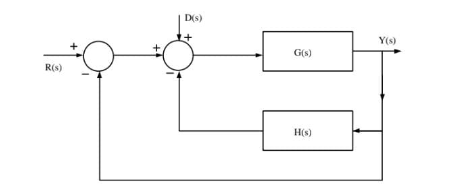
\includegraphics[width=\columnwidth]{2023/EC/42/figs/gate.png}
\end{figure}
\solution
\newpage


\item A causal, discrete time system is described by the difference equation $y[n] = 0.5 y[n-1] + x[n]$, for all $n$, where $y[n]$ denotes the output sequence and $x[n]$ denotes the input sequence. Which of the following statements is/are TRUE?
\begin{flushright}
\end{flushright}

\begin{enumerate}[label = (\alph*)]
	\item he system has an impulse response described by $0.5^{n} u[-n]$ where $u[n]$ is the  
unit step sequence. 		
	\item The system is stable in the bounded input, bounded output sense.
	\item The system has an infinite number of non-zero samples in its impulse response
	\item The system has a finite number of non-zero samples in its impulse response.
\end{enumerate}
\hfill(GATE BM 2023) \\
\solution
\newpage


\item 
\textbf{26.} A causal, discrete time system is described by the difference equation $y[n] = 0.5 y[n-1] + x[n]$, for all $n$, where $y[n]$ denotes the output sequence and $x[n]$ denotes the input sequence. Which of the following statements is/are TRUE?
\begin{flushright}
\hfill(GATE 2023 BM)
\end{flushright}

\begin{enumerate}[label = (\alph*)]
	\item he system has an impulse response described by $0.5^{n} u[-n]$ where $u[n]$ is the  
unit step sequence. 		
	\item The system is stable in the bounded input, bounded output sense.
	\item The system has an infinite number of non-zero samples in its impulse response
	\item The system has a finite number of non-zero samples in its impulse response.
\end{enumerate}
\solution
\newpage


\end{enumerate}

\chapter{Sequences}
\begin{enumerate}[label=\thechapter.\arabic*,ref=\thechapter.\theenumi]

\item Consider the discrete time signal $x\sbrak{n} = u\sbrak{-n+5} - u\sbrak{n+3}$, where
\[u\sbrak{n} = 
\begin{cases}
    1;n\geq0\\
    0;n<0
\end{cases}
\]
The smallest n for which $x\sbrak{n} = 0$ is?
\hfill(GATE IN 2023)
\\ \solution
\iffalse
\let\negmedspace\undefined
\let\negthickspace\undefined
\documentclass[journal,12pt,onecolumn]{IEEEtran}
\usepackage{cite}
\usepackage{amsmath,amssymb,amsfonts,amsthm}
\usepackage{algorithmic}
\usepackage{graphicx}
\usepackage{textcomp}
\usepackage{xcolor}
\usepackage{txfonts}
\usepackage{listings}
\usepackage{enumitem}
\usepackage{mathtools}
\usepackage{gensymb}
\usepackage{comment}
\usepackage[breaklinks=true]{hyperref}
\usepackage{tkz-euclide} % loads  TikZ and tkz-base
\usepackage{listings}
\usepackage[latin1]{inputenc}                                
\usepackage{color}                                            
\usepackage{array}                                            
\usepackage{longtable}                                       
\usepackage{calc}                                             
\usepackage{multirow}                                         
\usepackage{hhline}                                           
\usepackage{ifthen}                                           
\usepackage{lscape}
\usepackage{caption}
\usepackage{subcaption}


\newtheorem{theorem}{Theorem}[section]
\newtheorem{problem}{Problem}
\newtheorem{proposition}{Proposition}[section]
\newtheorem{lemma}{Lemma}[section]
\newtheorem{corollary}[theorem]{Corollary}
\newtheorem{example}{Example}[section]
\newtheorem{definition}[problem]{Definition}
%\newtheorem{thm}{Theorem}[section] 
%\newtheorem{defn}[thm]{Definition}
%\newtheorem{algorithm}{Algorithm}[section]
%\newtheorem{cor}{Corollary}
\newcommand{\BEQA}{\begin{eqnarray}}
\newcommand{\EEQA}{\end{eqnarray}}
\newcommand{\define}{\stackrel{\triangle}{=}}
\theoremstyle{remark}
\newtheorem{rem}{Remark}
%\bibliographystyle{ieeetr}

\begin{document}

%
\providecommand{\pr}[1]{\ensuremath{\Pr\left(#1\right)}}
\providecommand{\prt}[2]{\ensuremath{p_{#1}^{\left(#2\right)} }}        % own macro for this question
\providecommand{\qfunc}[1]{\ensuremath{Q\left(#1\right)}}
\providecommand{\sbrak}[1]{\ensuremath{{}\left[#1\right]}}
\providecommand{\lsbrak}[1]{\ensuremath{{}\left[#1\right.}}
\providecommand{\rsbrak}[1]{\ensuremath{{}\left.#1\right]}}
\providecommand{\brak}[1]{\ensuremath{\left(#1\right)}}
\providecommand{\lbrak}[1]{\ensuremath{\left(#1\right.}}
\providecommand{\rbrak}[1]{\ensuremath{\left.#1\right)}}
\providecommand{\cbrak}[1]{\ensuremath{\left\{#1\right\}}}
\providecommand{\lcbrak}[1]{\ensuremath{\left\{#1\right.}}
\providecommand{\rcbrak}[1]{\ensuremath{\left.#1\right\}}}
\newcommand{\sgn}{\mathop{\mathrm{sgn}}}
\providecommand{\abs}[1]{\left\vert#1\right\vert}
\providecommand{\res}[1]{\Res\displaylimits_{#1}} 
\providecommand{\norm}[1]{\left\lVert#1\right\rVert}
%\providecommand{\norm}[1]{\lVert#1\rVert}
\providecommand{\mtx}[1]{\mathbf{#1}}
\providecommand{\mean}[1]{E\left[ #1 \right]}
\providecommand{\cond}[2]{#1\middle|#2}
\providecommand{\fourier}{\overset{\mathcal{F}}{ \rightleftharpoons}}
\newenvironment{amatrix}[1]{%
  \left(\begin{array}{@{}*{#1}{c}|c@{}}
}{%
  \end{array}\right)
}
%\providecommand{\hilbert}{\overset{\mathcal{H}}{ \rightleftharpoons}}
%\providecommand{\system}{\overset{\mathcal{H}}{ \longleftrightarrow}}
        %\newcommand{\solution}[2]{\textbf{Solution:}{#1}}
\newcommand{\solution}{\noindent \textbf{Solution: }}
\newcommand{\cosec}{\,\text{cosec}\,}
\providecommand{\dec}[2]{\ensuremath{\overset{#1}{\underset{#2}{\gtrless}}}}
\newcommand{\myvec}[1]{\ensuremath{\begin{pmatrix}#1\end{pmatrix}}}
\newcommand{\mydet}[1]{\ensuremath{\begin{vmatrix}#1\end{vmatrix}}}
\newcommand{\myaugvec}[2]{\ensuremath{\begin{amatrix}{#1}#2\end{amatrix}}}
\providecommand{\rank}{\text{rank}}
\providecommand{\pr}[1]{\ensuremath{\Pr\left(#1\right)}}
\providecommand{\qfunc}[1]{\ensuremath{Q\left(#1\right)}}
        \newcommand*{\permcomb}[4][0mu]{{{}^{#3}\mkern#1#2_{#4}}}
\newcommand*{\perm}[1][-3mu]{\permcomb[#1]{P}}
\newcommand*{\comb}[1][-1mu]{\permcomb[#1]{C}}
\providecommand{\qfunc}[1]{\ensuremath{Q\left(#1\right)}}
\providecommand{\gauss}[2]{\mathcal{N}\ensuremath{\left(#1,#2\right)}}
\providecommand{\diff}[2]{\ensuremath{\frac{d{#1}}{d{#2}}}}
\providecommand{\myceil}[1]{\left \lceil #1 \right \rceil }
\newcommand\figref{Fig.~\ref}
\newcommand\tabref{Table~\ref}
\newcommand{\sinc}{\,\text{sinc}\,}
\newcommand{\rect}{\,\text{rect}\,}
%%
%       %\newcommand{\solution}[2]{\textbf{Solution:}{#1}}
%\newcommand{\solution}{\noindent \textbf{Solution: }}
%\newcommand{\cosec}{\,\text{cosec}\,}
%\numberwithin{equation}{section}
%\numberwithin{equation}{subsection}
%\numberwithin{problem}{section}
%\numberwithin{definition}{section}
%\makeatletter
%\@addtoreset{figure}{problem}
%\makeatother

%\let\StandardTheFigure\thefigure
\let\vec\mathbf

\bibliographystyle{IEEEtran}

\renewcommand{\thefigure}{\theenumi}
\renewcommand{\thetable}{\theenumi}
%\renewcommand{\theequation}{\theenumi}
Q:Which one of the options given is the inverse Laplace transform of $\frac{1}{s^3-s}$?\\
$u(t)$ denotes the unit-step function.
\begin{enumerate}[label=(\Alph*)]
\item $\left(-1+\frac{1}{2}e^-t+\frac{1}{2}e^t\right)u(t)$\\
\item $\left(\frac{1}{3}e^-t-e^t\right)u(t)$\\
\item $\left(-1+\frac{1}{2}e^{-(t-1)}+\frac{1}{2}e^{(t-1)}\right)u(t-1)$\\
\item $\left(-1-\frac{1}{2}e^{-(t-1)}-\frac{1}{2}e^{(t-1)}\right)u(t-1)$\\
\end{enumerate}
\hfill(GATE ME 2023)

%\end{document}

\newpage
\item Two sequences $x_1\sbrak{n} $ and $ x_2 \sbrak{n}$ are described as follows:
\begin{align}
x_1\sbrak{0} = x_2\sbrak{0} = 1\\
x_1\sbrak{1} = x_2\sbrak{2} = 2\\
x_1\sbrak{2} = x_2\sbrak{1} = 1
\end{align}
$x_1\sbrak{n} = x_2\sbrak{n} = 0$ for all $n<0$ and $n>2$\\
\\
If $x\sbrak{n}$ is obtained by convoluting $x_1\sbrak{n}$ with $x_2\sbrak{n}$, which of the following equations is/are TRUE?\\
\\
(A) $x\sbrak{2} = x\sbrak{3}$\\
\\
(B) $x\sbrak{1} = 2$\\
\\
(C) $x\sbrak{4} = 3$\\
\\
(D) $x\sbrak{2} = 5$\\
\hfill(GATE 2023 BM 47)
\solution
\input {2023/BM/47/Gate2023_Bm_47.tex}
\pagebreak
\item A series \brak{S} is given as S=1+3+5+7+9+..... The sum of the first 50 terms of S is \underline{\hspace{1in}}
\hfill(GATE 2023 BT 32)
\\ \solution
%% Run LaTeX on this file several times to get Table of Contents,
%% cross-references, and citations.

\documentclass[11pt]{book}
\usepackage{gvv-book}
\usepackage{gvv}
%\usepackage{Wiley-AuthoringTemplate}
\usepackage[sectionbib,authoryear]{natbib}% for name-date citation comment the below line
%\usepackage[sectionbib,numbers]{natbib}% for numbered citation comment the above line

%%********************************************************************%%
%%       How many levels of section head would you like numbered?     %%
%% 0= no section numbers, 1= section, 2= subsection, 3= subsubsection %%
\setcounter{secnumdepth}{3}
%%********************************************************************%%
%%**********************************************************************%%
%%     How many levels of section head would you like to appear in the  %%
%%				Table of Contents?			%%
%% 0= chapter, 1= section, 2= subsection, 3= subsubsection titles.	%%
\setcounter{tocdepth}{2}
%%**********************************************************************%%

%\includeonly{ch01}
\makeindex

\begin{document}

\frontmatter
%%%%%%%%%%%%%%%%%%%%%%%%%%%%%%%%%%%%%%%%%%%%%%%%%%%%%%%%%%%%%%%%
%% Title Pages
%% Wiley will provide title and copyright page, but you can make
%% your own titlepages if you'd like anyway
%% Setting up title pages, type in the appropriate names here:

\booktitle{Signal Processing }

\subtitle{Through GATE}

\AuAff{G. V. V. Sharma}


%% \\ will start a new line.
%% You may add \affil{} for affiliation, ie,
%\authors{Robert M. Groves\\
%\affil{Universitat de les Illes Balears}
%Floyd J. Fowler, Jr.\\
%\affil{University of New Mexico}
%}

%% Print Half Title and Title Page:
%\halftitlepage
\titlepage

%%%%%%%%%%%%%%%%%%%%%%%%%%%%%%%%%%%%%%%%%%%%%%%%%%%%%%%%%%%%%%%%
%% Copyright Page

\begin{copyrightpage}{2024}
%Title, etc
\end{copyrightpage}

% Note, you must use \ to start indented lines, ie,
% 
% \begin{copyrightpage}{2004}
% Survey Methodology / Robert M. Groves . . . [et al.].
% \       p. cm.---(Wiley series in survey methodology)
% \    ``Wiley-Interscience."
% \    Includes bibliographical references and index.
% \    ISBN 0-471-48348-6 (pbk.)
% \    1. Surveys---Methodology.  2. Social 
% \  sciences---Research---Statistical methods.  I. Groves, Robert M.  II. %
% Series.\\

% HA31.2.S873 2004
% 001.4'33---dc22                                             2004044064
% \end{copyrightpage}

%%%%%%%%%%%%%%%%%%%%%%%%%%%%%%%%%%%%%%%%%%%%%%%%%%%%%%%%%%%%%%%%
%% Only Dedication (optional) 

%\dedication{To my parents}

\tableofcontents

%\listoffigures %optional
%\listoftables  %optional

%% or Contributor Page for edited books
%% before \tableofcontents

%%%%%%%%%%%%%%%%%%%%%%%%%%%%%%%%%%%%%%%%%%%%%%%%%%%%%%%%%%%%%%%%
%  Contributors Page for Edited Book
%%%%%%%%%%%%%%%%%%%%%%%%%%%%%%%%%%%%%%%%%%%%%%%%%%%%%%%%%%%%%%%%

% If your book has chapters written by different authors,
% you'll need a Contributors page.

% Use \begin{contributors}...\end{contributors} and
% then enter each author with the \name{} command, followed
% by the affiliation information.

% \begin{contributors}
% \name{Masayki Abe,} Fujitsu Laboratories Ltd., Fujitsu Limited, Atsugi, Japan
%
% \name{L. A. Akers,} Center for Solid State Electronics Research, Arizona State University, Tempe, Arizona
%
% \name{G. H. Bernstein,} Department of Electrical and Computer Engineering, University of Notre Dame, Notre Dame, South Bend, Indiana; formerly of
% Center for Solid State Electronics Research, Arizona
% State University, Tempe, Arizona 
% \end{contributors}

%%%%%%%%%%%%%%%%%%%%%%%%%%%%%%%%%%%%%%%%%%%%%%%%%%%%%%%%%%%%%%%%
% Optional Foreword:

%\begin{foreword}
%\lipsum[1-2]
%\end{foreword}

%%%%%%%%%%%%%%%%%%%%%%%%%%%%%%%%%%%%%%%%%%%%%%%%%%%%%%%%%%%%%%%%
% Optional Preface:

%\begin{preface}
%\lipsum[1-1]
%\prefaceauthor{}
%\where{place\\
% date}
%\end{preface}

% ie,
% \begin{preface}
% This is an example preface.
% \prefaceauthor{R. K. Watts}
% \where{Durham, North Carolina\\
% September, 2004}

%%%%%%%%%%%%%%%%%%%%%%%%%%%%%%%%%%%%%%%%%%%%%%%%%%%%%%%%%%%%%%%%
% Optional Acknowledgments:

%\acknowledgments
%\lipsum[1-2]
%\authorinitials{I. R. S.}  

%%%%%%%%%%%%%%%%%%%%%%%%%%%%%%%%
%% Glossary Type of Environment:

% \begin{glossary}
% \term{<term>}{<description>}
% \end{glossary}

%%%%%%%%%%%%%%%%%%%%%%%%%%%%%%%%
%\begin{acronyms}
%\acro{ASTA}{Arrivals See Time Averages}
%\acro{BHCA}{Busy Hour Call Attempts}
%\acro{BR}{Bandwidth Reservation}
%\acro{b.u.}{bandwidth unit(s)}
%\acro{CAC}{Call / Connection Admission Control}
%\acro{CBP}{Call Blocking Probability(-ies)}
%\acro{CCS}{Centum Call Seconds}
%\acro{CDTM}{Connection Dependent Threshold Model}
%\acro{CS}{Complete Sharing}
%\acro{DiffServ}{Differentiated Services}
%\acro{EMLM}{Erlang Multirate Loss Model}
%\acro{erl}{The Erlang unit of traffic-load}
%\acro{FIFO}{First in - First out}
%\acro{GB}{Global balance}
%\acro{GoS}{Grade of Service}
%\acro{ICT}{Information and Communication Technology}
%\acro{IntServ}{Integrated Services}
%\acro{IP}{Internet Protocol}
%\acro{ITU-T}{International Telecommunication Unit -- Standardization sector}
%\acro{LB}{Local balance}
%\acro{LHS}{Left hand side}
%\acro{LIFO}{Last in - First out}
%\acro{MMPP}{Markov Modulated Poisson Process}
%\acro{MPLS}{Multiple Protocol Labeling Switching}
%\acro{MRM}{Multi-Retry Model}
%\acro{MTM}{Multi-Threshold Model}
%\acro{PASTA}{Poisson Arrivals See Time Averages}
%\acro{PDF}{Probability Distribution Function}
%\acro{pdf}{probability density function}
%\acro{PFS}{Product Form Solution}
%\acro{QoS}{Quality of Service}
%\acro{r.v.}{random variable(s)}
%\acro{RED}{random early detection}
%\acro{RHS}{Right hand side}
%\acro{RLA}{Reduced Load Approximation}
%\acro{SIRO}{service in random order}
%\acro{SRM}{Single-Retry Model}
%\acro{STM}{Single-Threshold Model}
%\acro{TCP}{Transport Control Protocol}
%\acro{TH}{Threshold(s)}
%\acro{UDP}{User Datagram Protocol}
%\end{acronyms}

\setcounter{page}{1}

\begin{introduction}
This book provides solutions to signal processing problems in GATE.

\end{introduction}

\mainmatter

\chapter{Harmonics}
\input{2023/harmonics.tex}
\chapter{Filters}
\input{2023/filters.tex}
\chapter{ Z-transform}
\chapter{Systems}
\input{2023/systems.tex}
\chapter{Sequences}
\input{2023/sequences.tex}
\chapter{Sampling}
\input{2023/sampling.tex}
\chapter{Contour Integration}
\input{2023/contour.tex}
\chapter{Laplace Transform}
 \input{2023/laplace.tex}
\chapter{Fourier transform}
 \input{2023/fourier.tex}
\backmatter
\appendix
\iffalse
\chapter{ Convolution}
\chapter{ Z-transform}
\fi
\latexprintindex

\end{document}

 

\pagebreak

\item For the signals x\brak{t} and y\brak{t} shown in the figure, $z\brak{t}=x\brak{t}*y\brak{t}$ is maximum at $t=T_1$. Then $T_1$ in seconds is .......... \brak{\text{Round off to the nearest integer}}
\solution
\pagebreak

\item A series of natural numbers F$_1$, F$_2$, F$_3$, F$_4$, F$_5$, F$_6$, F$_7$,....obeys F$_{n+1}$ = F$_n$ + F$_{n-1}$ for all integers n $\geq$ 2. If F$_6$ = 37, and F$_7$ = 60, then what is F$_1$?\\  
 \hfill[GATE CS 2023] \\
 \solution 
 \input{2023/CS/3/SS-GATE.tex}
 \pagebreak

 \item The Lucas sequence $L_{n}$is defined by the recurrence relation:\\
\begin{align*}
    L_{n}=L_{n-1}+L_{n-2}, for n\geq3
\end{align*}
with $L_{1}$=1 and $L_{2}$=3\\
Which one of the option given is TRUE?\\
\begin{enumerate}
    \item $L_{n}=\brak{\frac{1+\sqrt{5}}{2}}^n+\brak{\frac{1-\sqrt{5}}{2}}^n$
    \item $L_{n}=\brak{\frac{1+\sqrt{5}}{2}}^n-\brak{\frac{1-\sqrt{5}}{3}}^n$
    \item $L_{n}=\brak{\frac{1+\sqrt{5}}{2}}^n+\brak{\frac{1-\sqrt{5}}{3}}^n$
    \item $L_{n}=\brak{\frac{1+\sqrt{5}}{2}}^n-\brak{\frac{1-\sqrt{5}}{2}}^n$
\end{enumerate}
\hfill{(GATE 2023 CS 15)}\\
\solution
\iffalse
\let\negmedspace\undefined
\let\negthickspace\undefined
\documentclass[journal,12pt,twocolumn]{IEEEtran}
\usepackage{cite}
\usepackage{amsmath,amssymb,amsfonts,amsthm}
\usepackage{algorithmic}
\usepackage{graphicx}
\usepackage{textcomp}
\usepackage{xcolor}
\usepackage{txfonts}
\usepackage{listings}
\usepackage{enumitem}
\usepackage{mathtools}
\usepackage{gensymb}
\usepackage{comment}
\usepackage[breaklinks=true]{hyperref}
\usepackage{tkz-euclide} 
\usepackage{listings}
\usepackage{gvv}                                        
\def\inputGnumericTable{}                                 
\usepackage[latin1]{inputenc}                                
\usepackage{color}                                            
\usepackage{array}                                            
\usepackage{longtable}                                       
\usepackage{calc}                                             
\usepackage{multirow}                                         
\usepackage{hhline}                                           
\usepackage{ifthen}                                           
\usepackage{lscape}
\newtheorem{theorem}{Theorem}[section]
\newtheorem{problem}{Problem}
\newtheorem{proposition}{Proposition}[section]
\newtheorem{lemma}{Lemma}[section]
\newtheorem{corollary}[theorem]{Corollary}
\newtheorem{example}{Example}[section]
\newtheorem{definition}[problem]{Definition}
\newcommand{\BEQA}{\begin{eqnarray}}
\newcommand{\EEQA}{\end{eqnarray}}
\newcommand{\define}{\stackrel{\triangle}{=}}
\theoremstyle{remark}
\newtheorem{rem}{Remark}
\begin{document}
\parindent 0px
\bibliographystyle{IEEEtran}
\title{Assignment CS\_15Q}
\author{EE23BTECH11028 - Kamale Goutham$^{}$% <-this % stops a space
}
\maketitle
\newpage
\bigskip
\section*{Question}
The Lucas sequence $L_{n}$is defined by the recurrence relation:\\
\begin{align*}
    L_{n}=L_{n-1}+L_{n-2}, for n\geq3
\end{align*}
with $L_{1}$=1 and $L_{2}$=3\\
Which one of the option given is TRUE?\\
\begin{enumerate}
    \item $L_{n}=\brak{\frac{1+\sqrt{5}}{2}}^n+\brak{\frac{1-\sqrt{5}}{2}}^n$
    \item $L_{n}=\brak{\frac{1+\sqrt{5}}{2}}^n-\brak{\frac{1-\sqrt{5}}{3}}^n$
    \item $L_{n}=\brak{\frac{1+\sqrt{5}}{2}}^n+\brak{\frac{1-\sqrt{5}}{3}}^n$
    \item $L_{n}=\brak{\frac{1+\sqrt{5}}{2}}^n-\brak{\frac{1-\sqrt{5}}{2}}^n$
\end{enumerate}
\hfill{(GATE 2023 CS 15)}\\
\solution\\
\fi
Initial condition $L_{1}$=1 and $L_{2}$=3
\begin{align}
 L_{n}=L_{n-1}+L_{n-2}
\end{align}
Assume $L_{n+1}=x(n)$\\
\begin{align}
 x(n)=&[x(n-1)+x(n-2)-3]u(n-2)+u(n)+2u(n-1)\\
 X(z)=&z^{-1}(X(z)-1)+z^{-2}X(z)-3\frac{z^{-2}}{1-z^{-1}}+\frac{1}{1-z^{-1}}+2\frac{z^{-1}}{1-z^{-1}}\\
 X(z)&(1-z^{-1}-z^{-2})(1-z^{-1})=1+z^{-1}-2z^{-2}\\
 X(z)&=\frac{1+z^{-1}-2z^{-2}}{(1-z^{-1}-z^{-2})(1-z^{-1})}\\
 X(z)&=\frac{A}{1-z^{-1}}+\frac{B}{1-\alpha z^{-1}}+\frac{C}{1-\beta z^{-1}}
 \end{align}
 Where, $\alpha$ = $\dfrac{1 +\sqrt{5}}{2}$ and $\beta$ = $\dfrac{1 -\sqrt{5}}{2}$ \\
 
	\vspace{0.4cm}
 using partial fractions,
 \begin{align}
     X(z)=\frac{\alpha+2}{(\alpha-\beta)(1-\alpha z^{-1})}+\frac{\beta+2}{(\beta-\alpha)(1-\beta z^{-1})}
 \end{align}
 
	$a^n u(n)$
	$\xleftarrow[]{\hspace{0.4cm}{\mathcal{Z}}\hspace{0.1cm}}\xrightarrow[]{}$
	$\dfrac{1}{1 - a z^{-1}}$ \hspace{0.2cm} $\lvert \hspace{0.1cm} z \hspace{0.1cm}\rvert \hspace{0.1cm} \textgreater \hspace{0.1cm} \lvert \hspace{0.1cm} a \hspace{0.1cm} \rvert$
	
	\vspace{0.4cm}
	
	Substituting this result,
	
	\vspace{-0.5cm}
	
	\begin{align}
		x(n) &= \dfrac{\alpha+2}{(\alpha - \beta)} (\alpha^n u(n)) - \dfrac{\beta+2}{(\alpha - \beta)} (\beta^n u(n))\\
	    x(n) &= \dfrac{(5+\sqrt{5})(1 + \sqrt{5})^{n} - (5-\sqrt{5})(1 - \sqrt{5})^{n} }{2^{n+1} \sqrt{5}} u(n)\\
    	x(n) &= \dfrac{(1 + \sqrt{5})^{n+1} +(1 - \sqrt{5})^{n+1} }{2^{n+1}} u(n)
    \end{align}
$\therefore$ $L_{n} =\brak{\frac{1+\sqrt{5}}{2}}^n+\brak{\frac{1-\sqrt{5}}{2}}^n$
option 1 is correct.
\newpage
\begin{figure}[h]
  \centering
  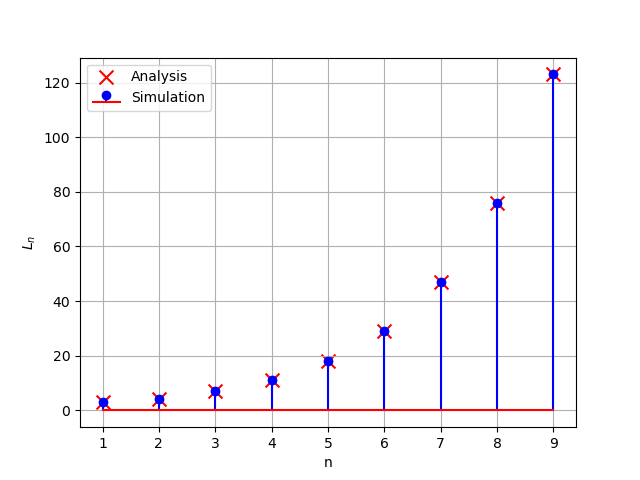
\includegraphics[width=\columnwidth]{2023/CS/15/figs/fig1.png}
  \caption{$L_{n}=\brak{\frac{1+\sqrt{5}}{2}}^n+\brak{\frac{1-\sqrt{5}}{2}}^n$}
\end{figure}

\pagebreak
\end{enumerate}

\chapter{Sampling}
\begin{enumerate}[label=\thechapter.\arabic*,ref=\thechapter.\theenumi]

\item An $8$ bit ADC converts analog voltage in the range of $0$ to $+5\, V$ to the corresponding digital code as per the conversion characteristics shown in figure. For $V_{in} = 1.9922\, V$, which of the following digital output, given in hex, is true?

\begin{figure}[!h]
    \centering
    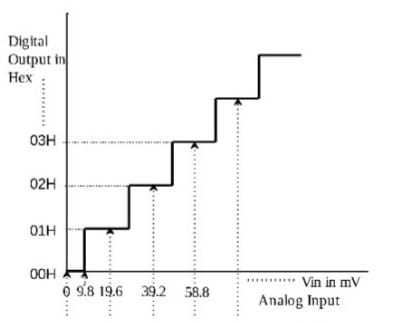
\includegraphics[width=\columnwidth]{2023/EE/40/figs/fig1.jpeg}
    \caption{}
    \label{fig:ADC}
\end{figure}
\begin{enumerate}[label=(\alph*)]
    \item $64H$
    \item $65H$
    \item $66H$
    \item $67H$
\end{enumerate} \hfill{GATE EE 40}\\

\solution
\iffalse
\let\negmedspace\undefined
\let\negthickspace\undefined
\documentclass[journal,12pt,twocolumn]{IEEEtran}
\usepackage{cite}
\usepackage{amsmath,amssymb,amsfonts,amsthm}
\usepackage{algorithmic}
\usepackage{graphicx}
\usepackage{textcomp}
\usepackage{xcolor}
\usepackage{txfonts}
\usepackage{listings}
\usepackage{enumitem}
\usepackage{mathtools}
\usepackage{gensymb}
\usepackage{comment}
\usepackage[breaklinks=true]{hyperref}
\usepackage{tkz-euclide} 
\usepackage{listings}
\usepackage{gvv}                                        
\def\inputGnumericTable{}                                
\usepackage[latin1]{inputenc}                            
\usepackage{color}                                       
\usepackage{array}                                       
\usepackage{longtable}                                   
\usepackage{calc}                              
\usepackage{tikz}
\usepackage{multirow}                                    
\usepackage{hhline}                                      
\usepackage{ifthen}                            
\usepackage{caption}
\usepackage{lscape}
\usepackage{amsmath}
\newtheorem{theorem}{Theorem}[section]
\newtheorem{problem}{Problem}
\newtheorem{proposition}{Proposition}[section]
\newtheorem{lemma}{Lemma}[section]
\newtheorem{corollary}[theorem]{Corollary}
\newtheorem{example}{Example}[section]
\newtheorem{definition}[problem]{Definition}
\newcommand{\BEQA}{\begin{eqnarray}}
\newcommand{\EEQA}{\end{eqnarray}}
\newcommand{\define}{\stackrel{\triangle}{=}}
\theoremstyle{remark}
\newtheorem{rem}{Remark}

\begin{document}

\bibliographystyle{IEEEtran}
\vspace{3cm}

\title{NCERT Math 11.9.2 Q8}
\author{EE23BTECH11009 - AROSHISH PRADHAN$^{*}$% <-this % stops a space
}
\maketitle
\newpage
\bigskip
\textbf{Question:} An $8$ bit ADC converts analog voltage in the range of $0$ to $+5\, V$ to the corresponding digital code as per the conversion characteristics shown in figure. For $V_{in} = 1.9922\, V$, which of the following digital output, given in hex, is true?

\begin{figure}[!h]
    \centering
    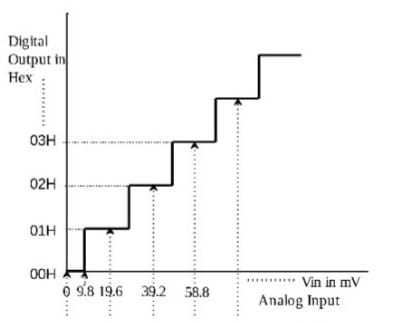
\includegraphics[width=\columnwidth]{2023/EE/40/figs/fig1.jpeg}
    \caption{}
    \label{fig:ADC_gate.ee.23.40}
\end{figure}
\begin{enumerate}[label=(\alph*)]
    \item $64H$
    \item $65H$
    \item $66H$
    \item $67H$
\end{enumerate}

\solution
\fi
\begin{table}[!h]
    \centering
    \resizebox{\columnwidth}{!}{\input{2023/EE/40/tables/table1}}
    \caption{Given Parameters}
    \label{tab:1_gate.ee.23.40}
\end{table}

Calculating the step-size:
\begin{align}
    \Delta V_{in} &= \frac{V_{max} - V_{min}}{2^n - 1}\\
    &= \frac{5 - 0}{2^8 - 1}\\
    &= \frac{5}{255}\\
   \implies V_{out} &= \frac{V_{in}}{\Delta V_{in}}\\
    &= \frac{1.9922 \times 255}{5}\\
    &= 101.59\\
    &\approx 102_{10}\\
    &= (66)_{H}
\end{align}
$\therefore$ correct answer is option (c).
\begin{figure}[!h]
    \centering
    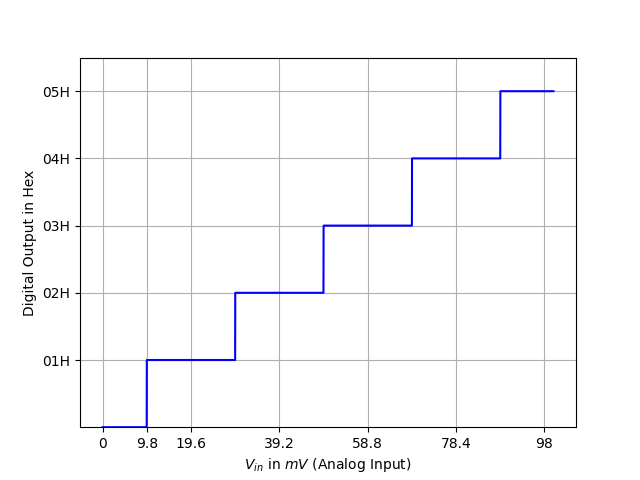
\includegraphics[width=\columnwidth]{2023/EE/40/figs/assign3.png}
    \caption{}
    \label{fig:ADC_plot_gate.ee.23.40}
\end{figure}

\newpage

\end{enumerate}

\chapter{Contour Integration}
\begin{enumerate}[label=\thechapter.\arabic*,ref=\thechapter.\theenumi]
\item The value of the contour integral, $\oint_C \frac{z + 2}{z^2 + 2z + 2} \, dz$, where the contour $C$ is $\{ z : |z + 1 - \frac{3}{2}i| = 1 \}$, taken in the counter clockwise direction, is \\

\begin{enumerate}
  \item[(A)] $-\pi(1+j) $
  \item[(B)] $\pi(1+j)$
  \item[(C)] $\pi(1-j) $
  \item[(D)] $-\pi(1-j)$
\end{enumerate}

\hfill{(GATE EC 2023)}\\
\solution
\item \textbf{Question:}
Consider the contour integral $\oint \frac{dz}{z^4 + z^3 - 2z^2}$, along the curve $|z| = 3$ oriented in the counterclockwise direction. If $\text{Res}[f, z_0]$ denotes the residue of $f(z)$ at the point $z_0$, then which of the following are TRUE? \\
\begin{itemize}
    \item (A) $\text{Res}[f, 0] = -\frac{1}{4}$
    \item (B) $\text{Res}[f, 1] = \frac{1}{3}$
    \item (C) $\text{Res}[f, -2] = -\frac{1}{12}$
    \item (D) $\text{Res}[f, 2] = -1$
\end{itemize}
\solution
\pagebreak
\end{enumerate}

\chapter{Laplace Transform}
 \begin{enumerate}[label=\thechapter.\arabic*,ref=\thechapter.\theenumi]

\item The number of zeroes of the polynomial $P(s) = s^3+2s^2+5s+80$ in the right side of the plane?\hfill(GATE IN 2023) \\

\solution
%% Run LaTeX on this file several times to get Table of Contents,
%% cross-references, and citations.

\documentclass[11pt]{book}
\usepackage{gvv-book}
\usepackage{gvv}
%\usepackage{Wiley-AuthoringTemplate}
\usepackage[sectionbib,authoryear]{natbib}% for name-date citation comment the below line
%\usepackage[sectionbib,numbers]{natbib}% for numbered citation comment the above line

%%********************************************************************%%
%%       How many levels of section head would you like numbered?     %%
%% 0= no section numbers, 1= section, 2= subsection, 3= subsubsection %%
\setcounter{secnumdepth}{3}
%%********************************************************************%%
%%**********************************************************************%%
%%     How many levels of section head would you like to appear in the  %%
%%				Table of Contents?			%%
%% 0= chapter, 1= section, 2= subsection, 3= subsubsection titles.	%%
\setcounter{tocdepth}{2}
%%**********************************************************************%%

%\includeonly{ch01}
\makeindex

\begin{document}

\frontmatter
%%%%%%%%%%%%%%%%%%%%%%%%%%%%%%%%%%%%%%%%%%%%%%%%%%%%%%%%%%%%%%%%
%% Title Pages
%% Wiley will provide title and copyright page, but you can make
%% your own titlepages if you'd like anyway
%% Setting up title pages, type in the appropriate names here:

\booktitle{Signal Processing }

\subtitle{Through GATE}

\AuAff{G. V. V. Sharma}


%% \\ will start a new line.
%% You may add \affil{} for affiliation, ie,
%\authors{Robert M. Groves\\
%\affil{Universitat de les Illes Balears}
%Floyd J. Fowler, Jr.\\
%\affil{University of New Mexico}
%}

%% Print Half Title and Title Page:
%\halftitlepage
\titlepage

%%%%%%%%%%%%%%%%%%%%%%%%%%%%%%%%%%%%%%%%%%%%%%%%%%%%%%%%%%%%%%%%
%% Copyright Page

\begin{copyrightpage}{2024}
%Title, etc
\end{copyrightpage}

% Note, you must use \ to start indented lines, ie,
% 
% \begin{copyrightpage}{2004}
% Survey Methodology / Robert M. Groves . . . [et al.].
% \       p. cm.---(Wiley series in survey methodology)
% \    ``Wiley-Interscience."
% \    Includes bibliographical references and index.
% \    ISBN 0-471-48348-6 (pbk.)
% \    1. Surveys---Methodology.  2. Social 
% \  sciences---Research---Statistical methods.  I. Groves, Robert M.  II. %
% Series.\\

% HA31.2.S873 2004
% 001.4'33---dc22                                             2004044064
% \end{copyrightpage}

%%%%%%%%%%%%%%%%%%%%%%%%%%%%%%%%%%%%%%%%%%%%%%%%%%%%%%%%%%%%%%%%
%% Only Dedication (optional) 

%\dedication{To my parents}

\tableofcontents

%\listoffigures %optional
%\listoftables  %optional

%% or Contributor Page for edited books
%% before \tableofcontents

%%%%%%%%%%%%%%%%%%%%%%%%%%%%%%%%%%%%%%%%%%%%%%%%%%%%%%%%%%%%%%%%
%  Contributors Page for Edited Book
%%%%%%%%%%%%%%%%%%%%%%%%%%%%%%%%%%%%%%%%%%%%%%%%%%%%%%%%%%%%%%%%

% If your book has chapters written by different authors,
% you'll need a Contributors page.

% Use \begin{contributors}...\end{contributors} and
% then enter each author with the \name{} command, followed
% by the affiliation information.

% \begin{contributors}
% \name{Masayki Abe,} Fujitsu Laboratories Ltd., Fujitsu Limited, Atsugi, Japan
%
% \name{L. A. Akers,} Center for Solid State Electronics Research, Arizona State University, Tempe, Arizona
%
% \name{G. H. Bernstein,} Department of Electrical and Computer Engineering, University of Notre Dame, Notre Dame, South Bend, Indiana; formerly of
% Center for Solid State Electronics Research, Arizona
% State University, Tempe, Arizona 
% \end{contributors}

%%%%%%%%%%%%%%%%%%%%%%%%%%%%%%%%%%%%%%%%%%%%%%%%%%%%%%%%%%%%%%%%
% Optional Foreword:

%\begin{foreword}
%\lipsum[1-2]
%\end{foreword}

%%%%%%%%%%%%%%%%%%%%%%%%%%%%%%%%%%%%%%%%%%%%%%%%%%%%%%%%%%%%%%%%
% Optional Preface:

%\begin{preface}
%\lipsum[1-1]
%\prefaceauthor{}
%\where{place\\
% date}
%\end{preface}

% ie,
% \begin{preface}
% This is an example preface.
% \prefaceauthor{R. K. Watts}
% \where{Durham, North Carolina\\
% September, 2004}

%%%%%%%%%%%%%%%%%%%%%%%%%%%%%%%%%%%%%%%%%%%%%%%%%%%%%%%%%%%%%%%%
% Optional Acknowledgments:

%\acknowledgments
%\lipsum[1-2]
%\authorinitials{I. R. S.}  

%%%%%%%%%%%%%%%%%%%%%%%%%%%%%%%%
%% Glossary Type of Environment:

% \begin{glossary}
% \term{<term>}{<description>}
% \end{glossary}

%%%%%%%%%%%%%%%%%%%%%%%%%%%%%%%%
%\begin{acronyms}
%\acro{ASTA}{Arrivals See Time Averages}
%\acro{BHCA}{Busy Hour Call Attempts}
%\acro{BR}{Bandwidth Reservation}
%\acro{b.u.}{bandwidth unit(s)}
%\acro{CAC}{Call / Connection Admission Control}
%\acro{CBP}{Call Blocking Probability(-ies)}
%\acro{CCS}{Centum Call Seconds}
%\acro{CDTM}{Connection Dependent Threshold Model}
%\acro{CS}{Complete Sharing}
%\acro{DiffServ}{Differentiated Services}
%\acro{EMLM}{Erlang Multirate Loss Model}
%\acro{erl}{The Erlang unit of traffic-load}
%\acro{FIFO}{First in - First out}
%\acro{GB}{Global balance}
%\acro{GoS}{Grade of Service}
%\acro{ICT}{Information and Communication Technology}
%\acro{IntServ}{Integrated Services}
%\acro{IP}{Internet Protocol}
%\acro{ITU-T}{International Telecommunication Unit -- Standardization sector}
%\acro{LB}{Local balance}
%\acro{LHS}{Left hand side}
%\acro{LIFO}{Last in - First out}
%\acro{MMPP}{Markov Modulated Poisson Process}
%\acro{MPLS}{Multiple Protocol Labeling Switching}
%\acro{MRM}{Multi-Retry Model}
%\acro{MTM}{Multi-Threshold Model}
%\acro{PASTA}{Poisson Arrivals See Time Averages}
%\acro{PDF}{Probability Distribution Function}
%\acro{pdf}{probability density function}
%\acro{PFS}{Product Form Solution}
%\acro{QoS}{Quality of Service}
%\acro{r.v.}{random variable(s)}
%\acro{RED}{random early detection}
%\acro{RHS}{Right hand side}
%\acro{RLA}{Reduced Load Approximation}
%\acro{SIRO}{service in random order}
%\acro{SRM}{Single-Retry Model}
%\acro{STM}{Single-Threshold Model}
%\acro{TCP}{Transport Control Protocol}
%\acro{TH}{Threshold(s)}
%\acro{UDP}{User Datagram Protocol}
%\end{acronyms}

\setcounter{page}{1}

\begin{introduction}
This book provides solutions to signal processing problems in GATE.

\end{introduction}

\mainmatter

\chapter{Harmonics}
\input{2023/harmonics.tex}
\chapter{Filters}
\input{2023/filters.tex}
\chapter{ Z-transform}
\chapter{Systems}
\input{2023/systems.tex}
\chapter{Sequences}
\input{2023/sequences.tex}
\chapter{Sampling}
\input{2023/sampling.tex}
\chapter{Contour Integration}
\input{2023/contour.tex}
\chapter{Laplace Transform}
 \input{2023/laplace.tex}
\chapter{Fourier transform}
 \input{2023/fourier.tex}
\backmatter
\appendix
\iffalse
\chapter{ Convolution}
\chapter{ Z-transform}
\fi
\latexprintindex

\end{document}

 

\newpage

\item The circuit shown in the figure is initially in the steady state with the switch K in open condition and $\overline{K}$ in closed condition. The switch K is closed and $\overline{K}$ is opened simultaneously at the instant $t = t_1$, where $t_1 > 0$. The minimum value of $t_1$ in milliseconds such that there is no transient in the voltage across the 100 $\mu F$ capacitor, is \rule{1cm}{0.15mm} (Round off to 2 decimal places) \hfill (GATE EE 2023)
\begin{circuitikz}[american]
   \draw (0,0) to [isource, l=1A] (0,4) ;
   \draw (0,0) to [short] (3,0) to [C = 0.01F] (3,4) to [short] (6,4) to [R = 100 $\Omega$] (6,2) to [L = 1H] (6,0) to [short] (9,0) to [R = 25 $\Omega$] (9,4) to [short] (6,4) ;
   \draw (3,0) to [short] (6,0) ;
   \draw (0,4) to [ospst = $S_1$] ++(3,0); 
   \draw (7.5,4) to [cspst = $S_2$] ++(0,-2);
   \draw (7.5,2) to [short] (6,2) ;
   \draw (3,4) to [short ,i = $i_c$] (3,3);
   
\end{circuitikz}


\newpage
\item $y=e^{mx}+e^{-mx}$ is the solution of which differential equation?
\begin{enumerate}[label=\textbf{\arabic*.}, font=\bfseries, align=left]
    \item $\frac{dy}{dx} - my = 0$ 
    \item $\frac{dy}{dx} + my = 0$ 
    \item $\frac{d^{2}y}{dx^{2}} + m^{2}y = 0$ 
    \item $\frac{d^{2}y}{dx^{2}} - m^{2}y = 0$ 
\end{enumerate} \hfill(GATE AG 2023)
\solution

\newpage
\item  A cascade control strategy is shown in the figure below. The transfer function between the output $(y)$ and the secondary disturbance $(d_2)$ is defined as  \\
$$G_{d2}(s)= \frac{y(s)}{d_2(s)}$$. 
Which one of the following is the CORRECT expression for the transfer function $G_{d2}(s)$? \\
\begin{figure}[h]
    \centering
    \includegraphics[scale=0.25]{2023/CH/44/figs/g44fig1.jpeg}
    \caption{ }
    \label{}
\end{figure}
\begin{enumerate}[label=\Alph*.]
\item $\frac{1}{(11s+21)(0.1s+1)}$ 
\item $\frac{1}{(s+1)(0.1s+1)}$
\item $\frac{(s+1)}{(s+2)(0.1s+1)}$
\item $\frac{(s+1)}{(s+1)(0.1s+1)}$
\end{enumerate} \hfill (GATE CH 2023)
\solution
\newpage
\item In the differential equation $\frac{dy}{dx} + \alpha x y = 0, \alpha$ is a positive constant. If $y = 1.0$ at
$x = 0.0$, and $y = 0.8$ at $x = 1.0$, the value of $\alpha$ is (rounded off to three decimal places).  \hfill(GATE CE 2023)
\solution

\newpage
\item The switch $S_1$ was closed and $S_2$ was open for a long time. At t=0,switch $S_1$ is opened and $S_2$ is closed,simultaneously. The value of $i_c(0^{+})$, in amperes, is . \hfill (GATE EC 2023)\\
\begin{circuitikz}[american]
   \draw (0,0) to [isource, l=1A] (0,4) ;
   \draw (0,0) to [short] (3,0) to [C = 0.01F] (3,4) to [short] (6,4) to [R = 100 $\Omega$] (6,2) to [L = 1H] (6,0) to [short] (9,0) to [R = 25 $\Omega$] (9,4) to [short] (6,4) ;
   \draw (3,0) to [short] (6,0) ;
   \draw (0,4) to [ospst = $S_1$] ++(3,0); 
   \draw (7.5,4) to [cspst = $S_2$] ++(0,-2);
   \draw (7.5,2) to [short] (6,2) ;
   \draw (3,4) to [short ,i = $i_c$] (3,3);
   
\end{circuitikz}

\newpage

\item The continuous time signal $x(t)$ is described by:
\begin{align}
x(t)=
    \begin{cases}
        1, & \text{if } 0\: {\displaystyle \leq }\:t\:{\displaystyle \leq }\:1\\
        0, & \text{elsewhere}
    \end{cases} 
\end{align}
If $y(t)$ represents $x(t)$ convolved with itself, which of the following options is/are TRUE?
\begin{enumerate}[label = \Alph*]
    \item $y(t)$ = 0 for all $t<0$\\
    \item $y(t)$ = 0 for all $t>1$\\
    \item $y(t)$ = 0 for all $t>3$\\
    \item $\int_{0.1}^{0.75} \frac{dy(t)}{dt}\: \text{dt} \neq 0$
\end{enumerate}
\solution
\newpage

\item The Z-transform of a discrete signal $x\brak{n}$ is
\begin{align}
X\brak{z}=\dfrac{4z}{\brak{z-\dfrac{1}{5}} \brak{z-\dfrac{2}{3}} \brak{z-3}} \text{ with ROC= }R
\end{align}
Which one of the following statements is TRUE?
\begin{enumerate}[label = (\alph*)]
     \item Discrete time Fourier transform of $x\sbrak{n}$ converges if $R$ is $|z|>3$\\
     \item Discrete time Fourier transform of $x\sbrak{n}$ converges if $ R$ is $\dfrac{2}{3}<|z|<3$\\
     \item Discrete time Fourier transform of $x\sbrak{n}$ converges if $R$ is such that $x\sbrak{n}$ is a left-sided sequence.\\
     \item Discrete time Fourier transform of $x\sbrak{n}$ converges if $R$ is such that $x\sbrak{n}$is a right-sided sequence.\\
 \end{enumerate} \hfill{GATE EE 2023}
 \solution
 \newpage
 
\item The phase margin of the transfer function $G(s) = \frac{2(1-s)}{(1+s)^2}$ is \rule{1cm}{0.15mm} degrees. (rounded off to the nearest integer). \hfill (GATE IN 2023)\\
\solution
\newpage
\item Consider the second-order linear differential equation
\[x^2\frac{d^2y}{dx^2}+x\frac{dy}{dx}-y=0, \; x\geq 1\]
with the initial conditions \[y(x=1)=6,\; \;\; \frac{dy}{dx}\big{|}_{x=1}=2.\]
Then the value of $y$ at $x=2$ is \rule{2cm}{0.1mm}.\\{\hfill{GATE ME 2023}}\\
\solution
\newpage
\item The transfer function of a measuring instrument is \\
$$G_m(s) = \frac{1.05}{2s+1}exp(-s)$$
At time $t = 0$, a step change of +1 unit is introduced in the input of this instrument.The time taken by the instrument to show an increase of 1 unit in its output is(rounded off to two decimal places).\\ \hfill (GATE CH 2023)
\solution
\item
The laplace transform of $x_1(t)$ = $e^{-t}u(t)$ is $X_1(s)$, where $u(t)$ is the unit step function. The laplace transform of $x_2(t) = e^tu(-t)$ is $X_2(s)$. Which one of the following statements is TRUE?
\begin{enumerate}
    \item The region of convergence of $X_1(s)$ is $Re(s) \geq 0$
    \item The region of convergence of $X_2(s)$ is confined to the left half-plane of s.
    \item The region of convergence of $X_1(s)$ is confined to the right half-plane of s.
    \item the imaginary axis in the s-plane is included in both the region of convergence of $X_1(s)$ and the region of convergence of $X_2(s)$.
\end{enumerate} \hfill(GATE BM 2023)\\
\solution
\newpage
\item Given that $\frac{dy}{dx}=2x+y$ and $y=1$,when $x=0$ Using Runge-Kutta fourth order method,the value of $y$ at $x=0.2$ is \hfill(GATE 2023 AG 50) \\
\solution

\item The magnitude and phase plots shown in the figure match with the transfer-
function
\begin{figure}[h]
    \centering
    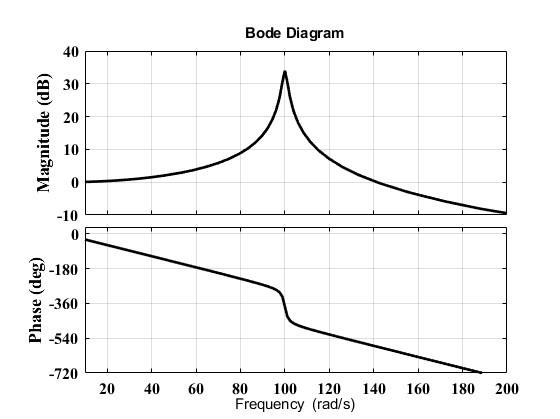
\includegraphics[width=\columnwidth]{2023/IN/43/figs/question.png}
\end{figure}\\
\begin{enumerate}
\item $\frac{10000}{s^2+2s+10000}$\\
\item $\frac{10000}{s^2+2s+10000}e^{-0.05s}$\\
\item $\frac{10000}{s^2+2s+10000}e^{-0.5\times10^{-12}s}$\\
\item $\frac{100}{s^2+2s+100}$
\end{enumerate}
\hfill{(GATE IN 2023)}
\solution

\item Which one of the options given is the inverse Laplace transform of $\frac{1}{s^3-s}$?\\
$u(t)$ denotes the unit-step function.
\begin{enumerate}[label=(\Alph*)]
\item $\left(-1+\frac{1}{2}e^-t+\frac{1}{2}e^t\right)u(t)$\\
\item $\left(\frac{1}{3}e^-t-e^t\right)u(t)$\\
\item $\left(-1+\frac{1}{2}e^{-(t-1)}+\frac{1}{2}e^{(t-1)}\right)u(t-1)$\\
\item $\left(-1-\frac{1}{2}e^{-(t-1)}-\frac{1}{2}e^{(t-1)}\right)u(t-1)$\\
\end{enumerate}
\hfill(GATE ME 2023)\\
\solution
\newpage
\end{enumerate}

\chapter{Fourier transform}
 \begin{enumerate}[label=\thechapter.\arabic*,ref=\thechapter.\theenumi]
    \item The discrete-time Fourier transform of a signal x\sbrak{n} is $X\brak{\Omega}=\brak{1+\cos{\Omega}}e^{-j\Omega}$. Consider that $x_{p}\sbrak{n}$ is a periodic signal of period $N=5$ such that
        \begin{align}
            x_p\sbrak{n}&=x[n],\text{for n= 0, 1, 2}\\
            &=0,\text{for n= 3, 4}
        \end{align}
        Note that $x_p\sbrak{n}=\sum_{k=0}^{N-1}a_{k}e^{j\frac{2\pi}{N}kn}$. The magnitude of the Fourier series coefficient $a_3$ is \rule{3cm}{0.15mm} \brak{\text{Round off to 3 decimal places}}.\hfill(GATE EE 2023)
        \solution
        \newpage

\item Let a frequency modulated (FM) signal : $ x(t) = A \cos(\omega_c t + k_f \int_{-\infty}^{t} m(\lambda) d\lambda)$ , where $ m(t) $is a message signal of bandwidth $ W $. It is passed through a non-linear system with output $y(t) = 2x(t) + 5(x(t))^2 $.
Let $B_T $denote the FM bandwidth. The minimum value of $ \omega_c $ required to recover $ x(t) $ from $ y(t) $ is:\\
\begin{enumerate}[label = (\Alph*)]
\item $B_T + W$ \\
\item $\dfrac{3}{2} B_T$ \\
\item $2B_T + W$ \\
\item $\dfrac{5}{2} B_T$ \\
\end{enumerate}

\solution
\newpage

\item Let an input $x[n]$ having discrete-time Fourier transform
$X(e^{j\Omega}) = 1 - e^{-j\Omega} + 2e^{-3j\Omega}$
be passed through an LTI system. The frequency response of the LTI system is 
$H(e^{j\Omega}) = 1 - \frac{1}{2} e^{-2j\Omega}$
The output $y[n]$ of the system is \\ \hfill(GATE EC 2023)
\solution 
\newpage
\item The Fourier transform $X(\omega)$ of $x(t) = e^{-t^2}$ is\\
Note:$\int_{-\infty}^{\infty} e^{-y^2} \,dy = \sqrt{\pi}$ \\  
A) $\sqrt{\pi} e^{\frac{\omega^2}{2}}$ \\
B) $\frac{e^{\frac{-\omega^2}{4}}}{2\sqrt{\pi}}$ \\
C) $\sqrt{\pi} e^{\frac{-\omega^2}{4}}$ \\
D) $\sqrt{\pi} e^{\frac{-\omega^2}{2}}$\\
\hfill Gate 2023 EC Question 28
\newpage

 \item Let $x(t) = 10 \cos(10.5 \omega t)$ be passed through an LTI system with impulse response $h(t) = \pi\left(\frac{\sin(\omega t)}{\pi t}\right)^2 \cos(10 \omega t)$ . The output of the system is:\\ \hfill(GATE EC 2023)
 \solution
 \newpage
 
 \item Q27) Let m\brak{\text{t}} be a strictly band-limited signal with bandwidth B and energy E. Assuming $\omega_0$ = 10B, the energy in the signal $\text{m}\brak{t}\text{cos}\brak{\omega_0\text{t}}$\\[1ex]

	\brak{A}\ $\frac{E}{4}$\\[1ex]

		\brak{B}\ $\frac{E}{2}$\\[1ex]

		\brak{C}\ $E$\\[1ex]

		\brak{D}\ $2E$ \qquad\qquad\qquad\quad\qquad\qquad\qquad\qquad\brak{\text{GATE EC 2023}}\\

\solution

\newpage

\item Consider a discrete-time signal with period $N=5$. Let the discrete-time Fourier series (DTFS) representation be $ x[n] = \sum\limits_{k=0}^{4} a_k e^{\frac{jk2\pi n}{5}} $where $a_0=1$, $a_1=3j$, $a_2=2j$, $a_3=-2j$, $a_4=-3j$. The value of the sum $\sum\limits_{n=0}^{4}x[n] \sin\left(\frac{4\pi n}{5}\right) $is\\
(A) -10\\
(B) 10\\
(C) -2\\
(D) 2\\
\hfill Gate 2023 EC 47
\solution
\pagebreak

\end{enumerate}

\backmatter
\appendix
\iffalse
\chapter{ Convolution}
\chapter{ Z-transform}
\fi
\latexprintindex

\end{document}

 

\newpage

\item Level \brak{h} in a steam boiler is controlled by manipulating the flow rate \brak{F} of the break-up(fresh) water using a proportional \brak{P} controller. The transfer function between the output and the manipulated input is   \\
$$ \frac{h\brak{s}}{F\brak{s}}=\frac{0.25\brak{1-s}}{s\brak{2s+1}} $$   \\
The measurement and the valve transfer functions are both equal to 1. A process engineer wants to tune the controller so that the closed loop response gives the decaying oscillations under the servo mode. Which one of the following is the CORRECT value of the controller gain to be used by the engineer? \\
\begin{enumerate}[label=(\alph*)]
    \item $0.25$
    \item $2$
    \item $4$
    \item $6$
\end{enumerate} \hfill{GATE CH 2023} \\

\solution
\newpage
\item \input{2023/ME/30/me30.tex}

\item A system has transfer function
 \[\frac{Y(s)}{X(s)}=\frac {s-\pi}{s+\pi}\]
 let $u(t)$ be the unit step function.The input $x(t)$ that results in a steady-state output $y(t)=sin(\pi t)$ is \underline{\quad}.\hfill (GATE IN 2023)\\
 \solution
 \newpage

 \item Consider the complex function
\[ f(z) = \frac{z^{2}\sin z}{(z-\pi)^4} \]
At \( z = \pi \), which of the following options is (are) correct?
\begin{enumerate}[label=\textbf{\arabic*.}, font=\bfseries, align=left]
    \item[(A)] The order of the pole is 4 
    \item[(B)] The order of the pole is 3 
    \item[(C)] The residue at the pole is \( \frac{\pi}{6} \)
    \item[(D)] The residue at the pole is \( \frac{2\pi}{3} \)
\end{enumerate}
\hfill (GATE PH 2023)\\
\solution
\newpage
\end{enumerate}
